\documentclass{standalone}
\usepackage{tikz}
\usetikzlibrary{patterns, positioning}


\begin{document}
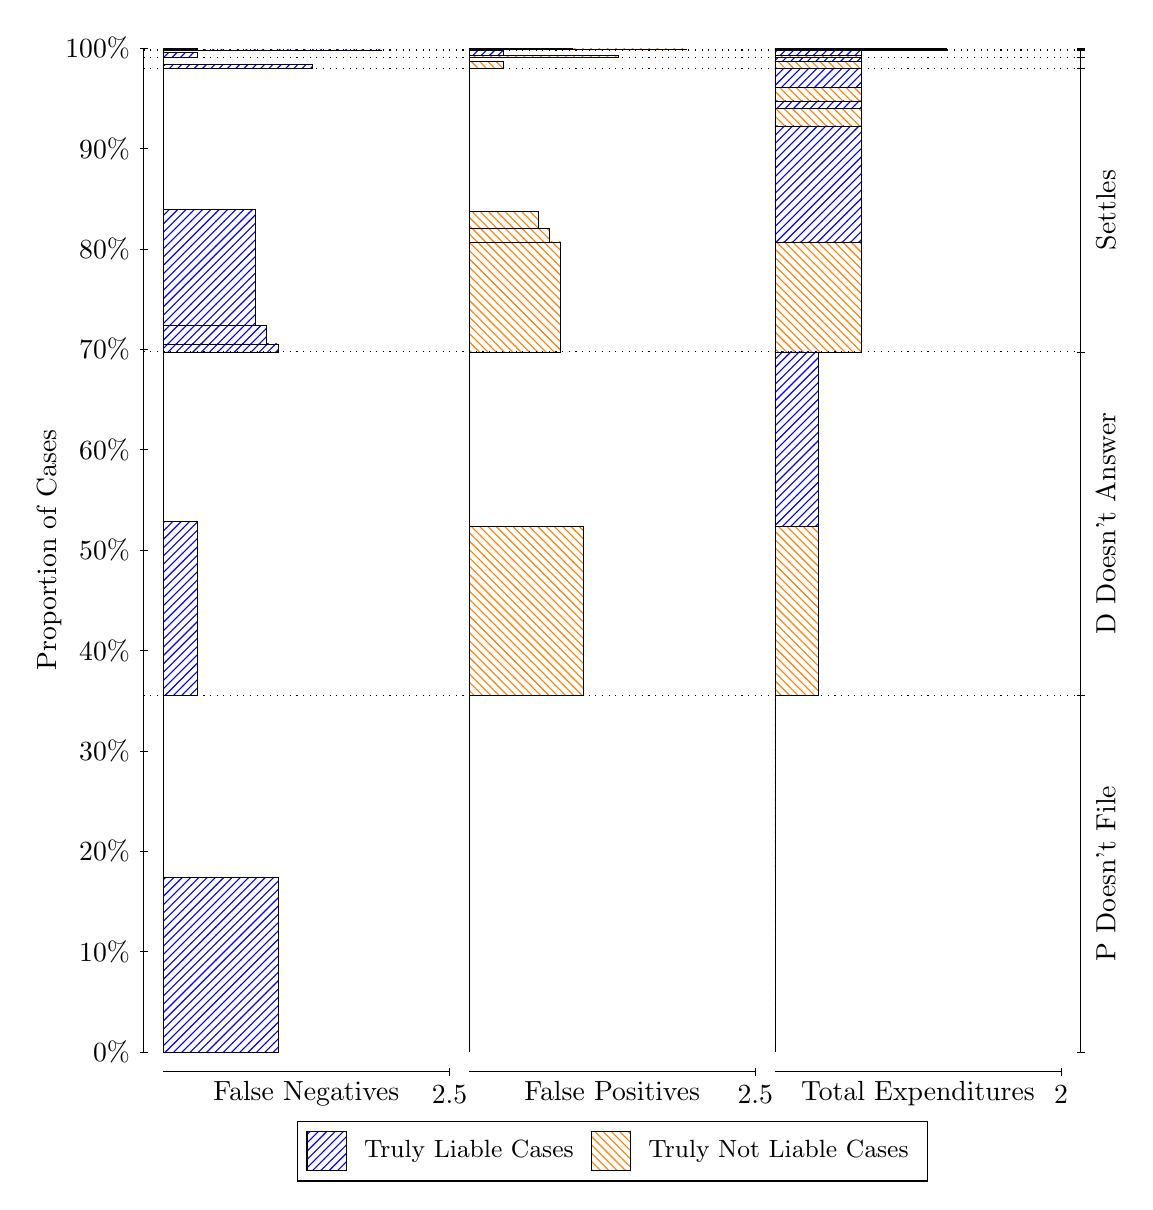
\begin{tikzpicture}
\draw[black, very thin] (1.5,1.75) -- (1.5,14.5);
\node[rotate=90, text=black, anchor=center] at (0.3, 8.125) {Proportion of Cases};
\draw[black, very thin] (1.45,1.75) -- (1.55,1.75);
\node[text=black, anchor=east] at (1.45, 1.75) {0\%};
\draw[black, very thin] (1.45,3.025) -- (1.55,3.025);
\node[text=black, anchor=east] at (1.45, 3.025) {10\%};
\draw[black, very thin] (1.45,4.3) -- (1.55,4.3);
\node[text=black, anchor=east] at (1.45, 4.3) {20\%};
\draw[black, very thin] (1.45,5.575) -- (1.55,5.575);
\node[text=black, anchor=east] at (1.45, 5.575) {30\%};
\draw[black, very thin] (1.45,6.85) -- (1.55,6.85);
\node[text=black, anchor=east] at (1.45, 6.85) {40\%};
\draw[black, very thin] (1.45,8.125) -- (1.55,8.125);
\node[text=black, anchor=east] at (1.45, 8.125) {50\%};
\draw[black, very thin] (1.45,9.4) -- (1.55,9.4);
\node[text=black, anchor=east] at (1.45, 9.4) {60\%};
\draw[black, very thin] (1.45,10.675) -- (1.55,10.675);
\node[text=black, anchor=east] at (1.45, 10.675) {70\%};
\draw[black, very thin] (1.45,11.95) -- (1.55,11.95);
\node[text=black, anchor=east] at (1.45, 11.95) {80\%};
\draw[black, very thin] (1.45,13.225) -- (1.55,13.225);
\node[text=black, anchor=east] at (1.45, 13.225) {90\%};
\draw[black, very thin] (1.45,14.5) -- (1.55,14.5);
\node[text=black, anchor=east] at (1.45, 14.5) {100\%};

\draw[black, very thin] (13.4,1.75) -- (13.4,14.5);
\draw[black, very thin] (13.35,1.75) -- (13.45,1.75);
\node[anchor=west] at (13.35, 1.75) {};
\draw[black, very thin] (13.35,6.2784) -- (13.45,6.2784);
\node[anchor=west] at (13.35, 6.2784) {};
\draw[black, very thin] (13.35,10.642) -- (13.45,10.642);
\node[anchor=west] at (13.35, 10.642) {};
\draw[black, very thin] (13.35,14.242) -- (13.45,14.242);
\node[anchor=west] at (13.35, 14.242) {};
\draw[black, very thin] (13.35,14.378) -- (13.45,14.378);
\node[anchor=west] at (13.35, 14.378) {};
\draw[black, very thin] (13.35,14.468) -- (13.45,14.468);
\node[anchor=west] at (13.35, 14.468) {};
\draw[black, very thin] (13.35,14.483) -- (13.45,14.483);
\node[anchor=west] at (13.35, 14.483) {};
\draw[black, very thin] (13.35,14.5) -- (13.45,14.5);
\node[anchor=west] at (13.35, 14.5) {};

\draw[black, very thin, pattern color=blue, pattern=north east lines] (1.75,1.75) rectangle (3.2033,3.9649);
\draw[black, very thin, pattern color=orange, pattern=north west lines] (1.75,3.9649) rectangle (1.75,6.2784);
\draw[black, very thin, pattern color=blue, pattern=north east lines] (1.75,6.2784) rectangle (2.186,8.4918);
\draw[black, very thin, pattern color=orange, pattern=north west lines] (1.75,8.4918) rectangle (1.75,10.642);
\draw[black, very thin, pattern color=blue, pattern=north east lines] (1.75,10.642) rectangle (3.2033,10.743);
\draw[black, very thin, pattern color=blue, pattern=north east lines] (1.75,10.743) rectangle (3.058,10.981);
\draw[black, very thin, pattern color=blue, pattern=north east lines] (1.75,10.981) rectangle (2.9127,12.455);
\draw[black, very thin, pattern color=orange, pattern=north west lines] (1.75,12.455) rectangle (1.75,14.242);
\draw[black, very thin, pattern color=blue, pattern=north east lines] (1.75,14.242) rectangle (3.6393,14.294);
\draw[black, very thin, pattern color=orange, pattern=north west lines] (1.75,14.294) rectangle (1.75,14.378);
\draw[black, very thin, pattern color=blue, pattern=north east lines] (1.75,14.378) rectangle (2.186,14.443);
\draw[black, very thin, pattern color=orange, pattern=north west lines] (1.75,14.443) rectangle (1.75,14.468);
\draw[black, very thin, pattern color=blue, pattern=north east lines] (1.75,14.468) rectangle (4.5113,14.475);
\draw[black, very thin, pattern color=orange, pattern=north west lines] (1.75,14.475) rectangle (1.75,14.483);
\draw[black, very thin, pattern color=blue, pattern=north east lines] (1.75,14.483) rectangle (2.186,14.494);
\draw[black, very thin, pattern color=orange, pattern=north west lines] (1.75,14.494) rectangle (1.75,14.5);
\draw[black, very thin, pattern color=orange, pattern=north west lines] (5.6333,1.75) rectangle (5.6333,4.0635);
\draw[black, very thin, pattern color=blue, pattern=north east lines] (5.6333,4.0635) rectangle (5.6333,6.2784);
\draw[black, very thin, pattern color=orange, pattern=north west lines] (5.6333,6.2784) rectangle (7.0867,8.429);
\draw[black, very thin, pattern color=blue, pattern=north east lines] (5.6333,8.429) rectangle (5.6333,10.642);
\draw[black, very thin, pattern color=orange, pattern=north west lines] (5.6333,10.642) rectangle (6.796,12.037);
\draw[black, very thin, pattern color=orange, pattern=north west lines] (5.6333,12.037) rectangle (6.6507,12.212);
\draw[black, very thin, pattern color=orange, pattern=north west lines] (5.6333,12.212) rectangle (6.5053,12.43);
\draw[black, very thin, pattern color=blue, pattern=north east lines] (5.6333,12.43) rectangle (5.6333,14.242);
\draw[black, very thin, pattern color=orange, pattern=north west lines] (5.6333,14.242) rectangle (6.0693,14.326);
\draw[black, very thin, pattern color=blue, pattern=north east lines] (5.6333,14.326) rectangle (5.6333,14.378);
\draw[black, very thin, pattern color=orange, pattern=north west lines] (5.6333,14.378) rectangle (7.5227,14.404);
\draw[black, very thin, pattern color=blue, pattern=north east lines] (5.6333,14.404) rectangle (6.0693,14.468);
\draw[black, very thin, pattern color=orange, pattern=north west lines] (5.6333,14.468) rectangle (6.0693,14.477);
\draw[black, very thin, pattern color=blue, pattern=north east lines] (5.6333,14.477) rectangle (5.6333,14.483);
\draw[black, very thin, pattern color=orange, pattern=north west lines] (5.6333,14.483) rectangle (8.3947,14.489);
\draw[black, very thin, pattern color=blue, pattern=north east lines] (5.6333,14.489) rectangle (6.9413,14.5);
\draw[black, very thin, pattern color=orange, pattern=north west lines] (9.5167,1.75) rectangle (9.5167,4.0635);
\draw[black, very thin, pattern color=blue, pattern=north east lines] (9.5167,4.0635) rectangle (9.5167,6.2784);
\draw[black, very thin, pattern color=orange, pattern=north west lines] (9.5167,6.2784) rectangle (10.062,8.429);
\draw[black, very thin, pattern color=blue, pattern=north east lines] (9.5167,8.429) rectangle (10.062,10.642);
\draw[black, very thin, pattern color=orange, pattern=north west lines] (9.5167,10.642) rectangle (10.607,12.037);
\draw[black, very thin, pattern color=blue, pattern=north east lines] (9.5167,12.037) rectangle (10.607,13.511);
\draw[black, very thin, pattern color=orange, pattern=north west lines] (9.5167,13.511) rectangle (10.607,13.729);
\draw[black, very thin, pattern color=blue, pattern=north east lines] (9.5167,13.729) rectangle (10.607,13.83);
\draw[black, very thin, pattern color=orange, pattern=north west lines] (9.5167,13.83) rectangle (10.607,14.004);
\draw[black, very thin, pattern color=blue, pattern=north east lines] (9.5167,14.004) rectangle (10.607,14.242);
\draw[black, very thin, pattern color=orange, pattern=north west lines] (9.5167,14.242) rectangle (10.607,14.326);
\draw[black, very thin, pattern color=blue, pattern=north east lines] (9.5167,14.326) rectangle (10.607,14.378);
\draw[black, very thin, pattern color=orange, pattern=north west lines] (9.5167,14.378) rectangle (10.607,14.404);
\draw[black, very thin, pattern color=blue, pattern=north east lines] (9.5167,14.404) rectangle (10.607,14.468);
\draw[black, very thin, pattern color=orange, pattern=north west lines] (9.5167,14.468) rectangle (11.697,14.477);
\draw[black, very thin, pattern color=blue, pattern=north east lines] (9.5167,14.477) rectangle (11.697,14.483);
\draw[black, very thin, pattern color=orange, pattern=north west lines] (9.5167,14.483) rectangle (11.697,14.489);
\draw[black, very thin, pattern color=blue, pattern=north east lines] (9.5167,14.489) rectangle (11.697,14.5);
\draw[black, dotted] (1.5,6.2784) -- (13.4,6.2784);
\draw[black, dotted] (1.5,10.642) -- (13.4,10.642);
\draw[black, dotted] (1.5,14.242) -- (13.4,14.242);
\draw[black, dotted] (1.5,14.378) -- (13.4,14.378);
\draw[black, dotted] (1.5,14.468) -- (13.4,14.468);
\draw[black, dotted] (1.5,14.483) -- (13.4,14.483);
\draw[black, very thin] (1.75,1.5) -- (5.3833,1.5);
\node[text=black, anchor=north] at (3.5667, 1.5) {False Negatives};
\draw[black, very thin] (5.3833,1.45) -- (5.3833,1.55);
\node[text=black, anchor=north] at (5.3833, 1.45) {2.5};

\draw[black, very thin] (5.6333,1.5) -- (9.2667,1.5);
\node[text=black, anchor=north] at (7.45, 1.5) {False Positives};
\draw[black, very thin] (9.2667,1.45) -- (9.2667,1.55);
\node[text=black, anchor=north] at (9.2667, 1.45) {2.5};

\draw[black, very thin] (9.5167,1.5) -- (13.15,1.5);
\node[text=black, anchor=north] at (11.333, 1.5) {Total Expenditures};
\draw[black, very thin] (13.15,1.45) -- (13.15,1.55);
\node[text=black, anchor=north] at (13.15, 1.45) {2};

\node[text=black, centered, rotate=90] at (13.72, 4.0142) {P Doesn't File};
\node[text=black, centered, rotate=90] at (13.72, 8.4604) {D Doesn't Answer};
\node[text=black, centered, rotate=90] at (13.72, 12.442) {Settles};





\draw (7.449999999999999,1.5) node[draw=none] (baseCoordinate) {};
\begin{scope}[align=center]
        \matrix[scale=0.5, draw=black, below=0.5cm of baseCoordinate, nodes={draw}, column sep=0.1cm]{
            \node[rectangle, draw, minimum width=0.5cm, minimum height=0.5cm, pattern color=blue, pattern=north east lines] {}; &
            \node[draw=none, font=\small, text=black] (B) {Truly Liable Cases}; &
            \node[rectangle, draw, minimum width=0.5cm, minimum height=0.5cm, pattern color=orange, pattern=north west lines] {}; &
            \node[draw=none, font=\small, text=black] (B) {Truly Not Liable Cases}; \\
            };
\end{scope}

\end{tikzpicture}
\end{document}